\section{Teori}
For å beskrive bevegelsen til sylinderen kan man bruke Newtons andre lov i tangentiell retning.
Man kan da finne et uttrykk for \(\ddot{\phi}\) gitt ved \(\dot{\phi}\) og \(\phi\). 
Denne differensialligningen inneholder også de tre dempekreftene \(f_S\), \(f_D\) og \(f_R\), 
som henholdsvis inneholder diverse dempekrefter, luftmotstand og rullefriksjon.

\begin{align}
	\vec{f_S} & = -\tilde{\delta} \vec{v} 			\\
	\vec{f_D} & = -\tilde{\beta}|\vec{v}|^2\hat{v}  \\
	\vec{f_R} & = -|\vec{f_R}|\hat{v}				
\end{align}

Her er \(\tilde{\delta}\) \text{dempingskonstanten}, \(\tilde{\beta}\) \text{dragkoeffisienten}.
Det kan vises at \(F_R\) kan uttrykkes ved

\begin{equation}
	|f_R|\text{sgn}\dot{\phi} =
	m\left[
		cl\ddot{\phi}+\frac{d}{r}
		\left(l\dot{\phi}^2 + g\cos\phi\right)
		\text{sgn }\dot{\phi}
	\right]
\end{equation}

Ved å bruke Newtons andre lov på den rullende sylinderen 
og bruke ligningen for \(f_R\) kommer man frem til følgende uttrykk:

\begin{equation}
	\begin{split}
		\label{ODE}	
		\ddot{\phi} = 	
		&- \omega_0^2\sin\phi - 2\delta\dot{\phi}	\\
		&- \frac{\pi\phi_R}{2\omega_0}
		\left(\omega_0^2\cos\phi + \gamma\dot{\phi}^2\right) \text{sgn } \dot{\phi} \\
		&- \beta \frac{3\pi}{4\omega_0}\dot{\phi}^2\text{sgn }\dot{\phi} 
	\end{split}
\end{equation}

Her er størrelsene \(\delta\), \(\beta\) og \(\phi_R\) skalerte versjoner av 
\(\tilde{\delta}\), \(\tilde{\beta}\) og \(d\), der \(d\) er armen til normalkraften (se figur \ref{Fig System}).
Disse er definert slik:
\begin{subequations}
    \begin{align}
        \delta & = \gamma\frac{\tilde{\delta}}{2m} \\
        \beta & = \frac{4\gamma}{3\pi}\frac{\omega_0l}{m}\tilde{\beta} \\
        \phi_R & = \frac{d}{r}\frac{2\omega_0}{\pi}
    \end{align}
\end{subequations}

Å løse differensialligninger eksakt vil i de fleste tilfeller være svært vanskelig eller umulig.
Likevel kan man løse \eqref{ODE} i noen grensetilfeller. Ved å bare se på \(\phi << 1\) vil man kunne
bruke approksimasjonene 
\(\sin(\phi) = \phi + \mathcal{O}(\phi^3) \approx \phi\) og 
\(\cos(\phi) = 1 + \mathcal{O}(x^2) \approx 1\).
I tillegg vil man kunne finne eksakte løsninger ved å sette to av \(\delta\), \(\beta\) og \(\phi_R\) lik 0.
\par
Selv om man i noen tilfeller kan finne analytiske løsninger 
vil det i mange tilfeller være mer hensiktsmessig å løse differensialligningen numerisk.
\eqref{ODE} er en ordinær differensialligning av andre orden. 
Denne kan skrives som to koblede førsteordens ordinære differensialligninger ved å innføre \(u = \dot{\phi}\):

\begin{subequations}
	\begin{align}
		\dd{\phi}{t} & = u \\
		\dd{u}{t}    & = f(\phi, u)
	\end{align}
\end{subequations}

Dette ligningssettet kan løses diskret ved bruk av Eulers metode. 
Man løser da

\begin{subequations}
	\begin{align}
		\label{Newton}
		\phi_{i+1} & = \phi_i + u_i \Delta{t} \\
		u_{i+1}    & = u_i + f(\phi_i, u_i) \Delta {t} 
	\end{align}
	for en valgt \(\Delta t\) og med startverdiene \(\phi_0\) og \(u_0 = \dot{\phi_0}\)
\end{subequations}.

Da Eulers metode ofte fører til systematisk avvik er det bedre å bruke Crank-Nicholson-metoden, som man kan finne i labheftet.

\begin{figure}[h] 
    \begin{center}
        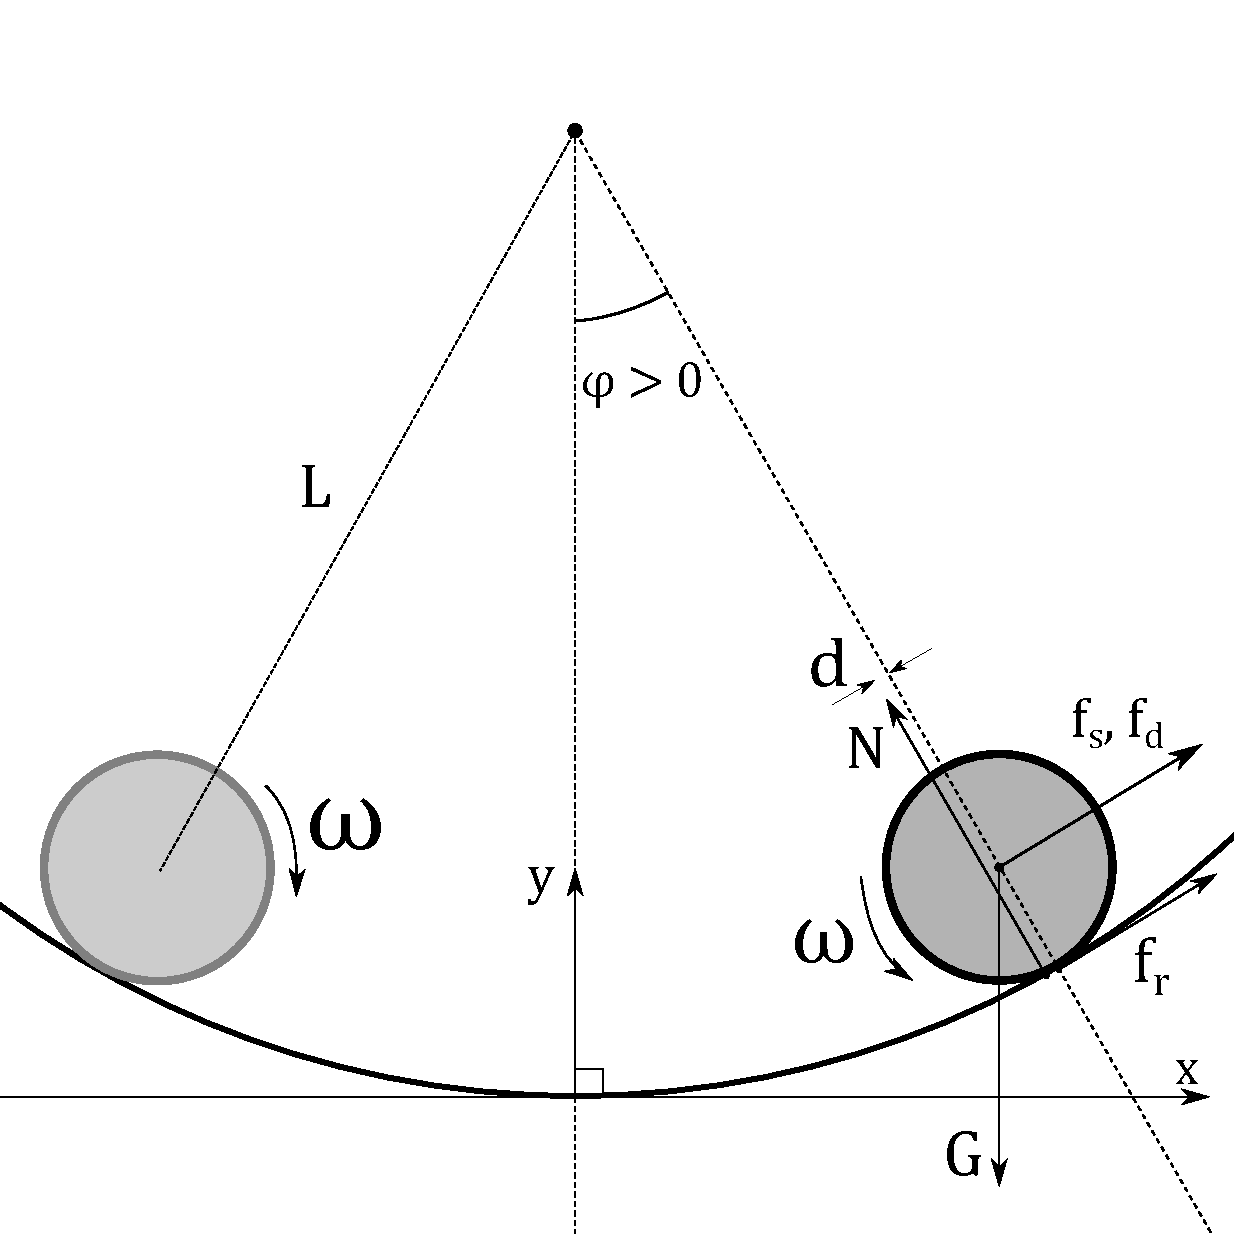
\includegraphics[width=0.4\textwidth]{img/drawing2}
    \end{center}
    \caption{Skisse av system.}
    \label{Fig System}
\end{figure}

\begin{figure}[h] 
    \begin{center}
        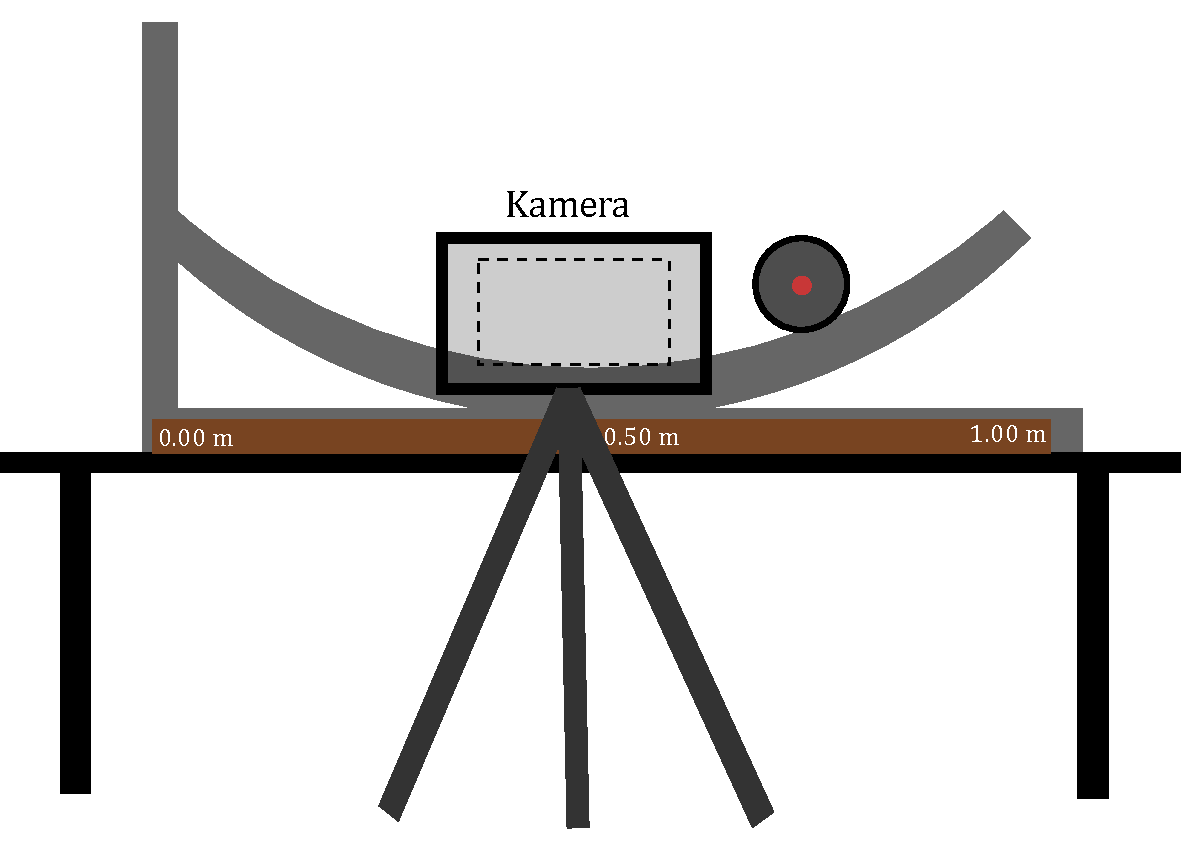
\includegraphics[width=0.4\textwidth]{img/skisse}
    \end{center}
    \caption{Skisse av oppsett.}
    \label{Fig Oppsett}
\end{figure}

